\documentclass{article}
\usepackage{tikz}

\begin{document}

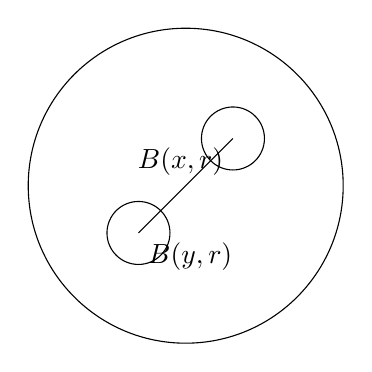
\begin{tikzpicture}[scale=2]
    % Draw the large circle
    \draw (0,0) circle (1);
    
    % Draw the two smaller circles with labels
    \draw (0.3,0.3) circle (0.2) node[below left] {$B(x,r)$};
    \draw (-0.3,-0.3) circle (0.2) node[below right] {$B(y,r)$};
    
    % Draw the connecting line between the two smaller circles
    \draw (0.3,0.3) -- (-0.3,-0.3);
\end{tikzpicture}

\end{document}